% !TEX TS-program = Xelatex
% !TEX encoding = UTF-8 Unicode

\documentclass[UTF8]{ctexart}
\usepackage{amsmath}
\usepackage[bottom]{footmisc}
\usepackage{geometry}
\usepackage{graphicx}
\usepackage{figsize}\usepackage[separate-uncertainty = true]{siunitx}
\usepackage{tabu}
\geometry{left=0.7in,right=0.7in,bottom=0.7in,top=0.7in}

\title{实验七:测量误差与数据处理}
\author{朱寅杰 1600017721}
\date{2017年10月20日}

\begin{document}

\maketitle

\section{实验数据}

\subsection{钢杯体积的测量}

实验时使用游标卡尺测量出钢杯的外径$R$、内径$r$、(外)高度$H$与(内)深度$h$,从而计算出钢杯的体积$V=\pi(R^2H-r^2h)/4$。

游标卡尺量程为\SI{12.5}{\cm},最小分度为\SI{0.05}{\mm},读数时估读到\SI{0.01}{\mm}。仪器的零点没有偏差,其极限误差取$e=\SI{0.005}{\cm}$。各数据均在不同方向上测量六次,取平均值作为测量结果,并计算几次测量的样本准偏差$\sigma_N=\sqrt{\sum (x_i-\bar{x})^2/(N-1)}$。从样本标准差估计出平均值偏离真值的标准差$\sigma_{\bar{N}}=\sigma_N/\sqrt{N}$,作为平均值不确定度的估计,再将仪器允差按$\sigma=e/\sqrt{3}$合成入最终测量结果的不确定度中$\sigma=\sqrt{\sigma_{\bar{N}}^2+e^2/3}$。

\noindent
\begin{tabu} to \linewidth {X[2]|X X X X X X|X[2] X[2]|X[2]}
\hline
待测量& 1&  2&  3&  4&  5&  6&  平均值$\bar{x}$\footnotemark[1]&标准差$\sigma_{\bar{N}}$&不确定度$\sigma$ \\
\hline
外径$R$/cm&	2.800&	2.803&	2.805&	2.803&	2.804&	2.805&	2.803333333&	0.000760117&	0.002985148
\\
内径$r$/cm&	1.995&	1.999&	1.985&	2.000&	1.997&	1.995&	1.995166667&	0.00219722&	0.003627825
\\
高$H$/cm&	4.469&	4.474&	4.471&	4.470&	4.474&	4.469&	4.471166667&	0.000945751&	0.003037726
\\
深$h$/cm&	4.255&	4.279&	4.262&	4.258&	4.264&	4.268&	4.264333333&	0.003470511&	0.004514175
\\
\hline
\end{tabu}

\footnotetext[1]{所有数据处理计算过程中的中间量为方便起见均保留至机器默认精度,在最终结果中才按照不确定度截取有效数字位数,后面的数据表与最小二乘法的中间算式中也采取同样的做法,还望老师谅解。}

根据计算出的不确定度,确定各测量结果的有效数字位数。有
\begin{gather}
   R=\SI{2.803(3)}{\cm} \\
   r=\SI{1.995(4)}{\cm} \\
   H=\SI{4.471(3)}{\cm} \\
   h=\SI{4.264(5)}{\cm}
\end{gather}

然后根据$V=\pi(R^2H-r^2h)/4$计算出钢杯的体积,并且估算其不确定度。按照复合函数不确定度合成的原则,有
\begin{equation*}
  \sigma_V=\sqrt{\sum(\frac{\partial V}{\partial x_i}\sigma_{x_i})^2}=\sqrt{(2RH\sigma_R)^2+(2rh\sigma_r)^2+(R^2\sigma_H)^2+(r^2\sigma_h)^2}=\SI{0.0797}{\cm^3}
\end{equation*}

故而$V=\pi(R^2H-r^2h)/4=\SI{14.26(8)}{\cm^3}$。

从数据表中可以看出,仪器允差对$R$、$r$、$H$的不确定度的贡献$e/\sqrt{3}=\SI{0.0029}{\cm}$大于随机误差的贡献,而对$h$不确定度的贡献小于随机误差。实验时我也感到$h$比起另几个量确实难测一些,从此分析看实验对$h$的测量的质量也确实不如其他量。

\subsection{钢珠体积的测量}
使用螺旋测微器测量小钢珠的直径$d$,并计算其体积$V=\pi d^3/6$。所使用的螺旋测微器量程为\SI{25}{\mm},零点位置在\SI{0.019}{\mm}处,鼓轮上最小刻度为\SI{0.01}{\mm},读数时估读到\SI{0.001}{\mm}。仪器的极限误差取为$e=\SI{0.004}{\mm}$。和上一例一样测量六次,计算平均值与样本标准差,从而求出平均值的标准差,再与仪器的极限误差合成得到钢珠直径的不确定度。数据记录处理如下表。

\noindent
\begin{tabu} to \linewidth {X|X X X X X X|X X[1.8]|X[1.8]}
\hline
& 1&  2&  3&  4&  5&  6&  平均值&标准差$\sigma_{\bar{N}}$&不确定度$\sigma$ \\
\hline
$d$/cm &12.728&12.729&12.730&12.729&12.727&12.728&12.7285&0.000428&0.002349\\
\hline
\end{tabu}

从计算出的不确定度确定$d$应取的有效位数,$d=\SI{12.729(2)}{\mm}$。考虑螺旋测微器零点的修正,有$d=\SI{12.710(2)}{\mm}$,从而计算出$V=\pi d^3/6$,并估计出$\sigma_V=(\partial V/\partial d)\sigma_d=\pi d^2 \sigma_d/2=\SI{0.596}{\mm^3}$。故而有$V=\pi d^3/6=\SI{1074.9(6)}{\mm^3}$。

从数据表中可以看出,仪器允差对$d$的不确定度的贡献$e/\sqrt{3}=\SI{0.0023}{\mm}$远大于随机误差的贡献,证明多次测量已经有效地减小了随机误差的影响。

\section{作业题}
\subsection{}
\SI{0.0001}{cm}是一位有效数字,\SI{1.000}{s}是四位有效数字,\SI{2.7e25}{\joule}是两位有效数字,\SI{980.120}{cm.s^{-2}}是六位有效数字。
\subsection{}
今已知$a=\SI{9.9}{\cm}$,$b=\SI{999.9}{\cm}$,$c=ab/(b-a)$。取$a$与$b$的极限误差$e_a=e_b=\SI{0.05}{\cm}$,有$(\partial c/\partial a)=\frac{b^2}{(a-b)^2}=1.0201$,$(\partial c/\partial b)=-\frac{a^2}{(a-b)^2}=\num{-1e-4}$,故而$e_c=\lvert e_a\partial c/\partial a\rvert+\lvert e_b\partial c/\partial b\rvert=\SI{0.05101}{\cm}$。因此$c$的有效位数留到\SI{0.1}{\cm}位,$c=\SI{10.0}{\cm}$。

今已知$x=9.24, y=\exp{(-x^2)}$,故取$e_x=0.005$,有 $e_y=\lvert y'(x)e_x\rvert=2xye_x=\num{7.7e-39}$。故$y=\exp{(-x^2)}=\num{8.3e-38}$。

今已知$x=56.7, y=\ln{x}$,故取$e_x=0.05$,有 $e_y=\lvert y'(x)e_x\rvert=e_x/x=\num{8.8e-4}$。故$y=\ln{x}=\num{4.038}$。

今已知$x=\ang{9;24;}, y=\cos{x}$,故取$e_x=\ang{0;0;30}$,有 $e_y=\lvert y'(x)e_x\rvert=\sin{x}e_x=\num{2.4e-5}$。故$y=\cos{x}=\num{0.98657}$。
\subsection{}
已知$\rho=\rho_0m_1/(m_1-m_2)$,则$\sigma_{\rho}=\sqrt{(\sigma_{m_1}\partial\rho/\partial m_1)^2+(\sigma_{m_2}\partial\rho/\partial m_2)^2}=\rho_0\sqrt{(\sigma_{m_1}m_2)^2+(\sigma_{m_2}m_1)^2}/(m_1-m_2)^2$。

已知$y=\ln{ab/(a+b)}$,则$\sigma_y=\sqrt{(\sigma_{a}\partial y/\partial a)^2+(\sigma_b\partial y/\partial b)^2}=\sqrt{(b\sigma_a/a)^2+(a\sigma_b/b)^2}/(a+b)$。
\subsection{}
为测出$L$有三种方案,一种是$L=L_1+d_1/2+d_2/2$,一种是$L=L_2-d_1/2-d_2/2$,还有一种是$L=L_1/2+L_2/2$。第一种$\sigma_L^2=\sigma_{L_1}^2+(\sigma_{d_1}^2+\sigma_{d_2}^2)/4=\SI{0.825}{\micro\meter\squared}$,第二种$\sigma_L^2=\sigma_ {L_2}^2+(\sigma_{d_1}^2+\sigma_{d_2}^2)/4=\SI{1.185}{\micro\meter\squared}$,第三种$\sigma_L^2=\sigma_{L_1}^2/4+\sigma_{L_2}^2/4=\SI{0.41}{\micro\meter\squared}$。比较三种测法知第三种测法最优。
\subsection{}
对平板表面面积先作一估算,$A=L_1L_2-\pi(d_1^2+d_2^2)/4\doteq\SI{62.84}{\cm\squared}$,不确定度不超过0.5\%即要求$e_A\leq\SI{0.314}{\cm\squared}$。估算$e_L=L_2e_{L_1}+L_1e_{L_2}+\pi d_1e_{d_1}/2+\pi d_2e_{d_2}/2=\SI{0.200}{\cm\squared}+\pi d_2e_{d_2}/2$,故这要求$e_{d_2}\leq\SI{0.91}{\cm}$,因此不必再对小孔再做测量,粗测已经足够满足精度的要求。
\subsection{}
使用$g=2h/t^2$测重力加速度,其中$h$由于钢尺的热胀会偏小$\SI{1e-5}{K}\times\SI{10}{K}=\num{1e-4}$,而$t$由于停表慢了万分之一会偏小\num{1e-4}。将二者的影响叠加,最终测出的$g$会比真值偏大\num{1e-4},即从\SI{980.00}{\cm\per\second\squared}变为\SI{980.01}{\cm\per\second\squared}。

对于单摆的周期,如果考虑摆幅较大时的非线性项,那么为了使周期的准确度好于0.5\%,摆角不应超过\ang{16};为了使周期的准确度好于0.05\%,摆角不应超过\ang{5}。
\subsection{测量空气中声速}
测出相位相差$2\pi$的点的位置$y_i$,有$y_i=b_0+i\lambda, i=1,2,3...$。$y_i$的值如下表:

\noindent\begin{tabu} to \linewidth {X|X X X X X X X X X X}
\hline
$i$ &1&2&3&4&5&6&7&8&9&10\\
\hline
$y_i/\si{\mm}$&27.257 &36.012 &44.973 &54.115 &62.630 &71.310 &80.068 &88.878 &97.200 &106.128\\
\hline
\end{tabu}

对$y_i$作最小二乘法拟合,根据书上公式(7.14)、(7.16)、(7.19)有
\begin{gather}
  \lambda=\frac{6}{n^2-1}(2\sum\limits_ {j=1}^{n}jy_j/n-(n+1)\bar{y})=6(2\times 439.925-11\times66.8571)/99=\SI{8.7528}{\mm}\\
  r=\frac{2\sum\limits_ {j=1}^{n}jy_j/n-(n+1)\bar{y}}{\sqrt{(\bar{y^2}-\bar{y}^2)(n^2-1)/3}}=0.99997\\
  \sigma_{\lambda,statistical}=\lambda\sqrt{\frac{1/r^2-1}{n-2}}=\SI{0.024}{\mm}
\end{gather}
以上这个标准差计算的是由回归分析得到的$\lambda$的不确定度的估计,还需合成入尺子的允差$e=\SI{0.005}{\mm}$与用示波器等判断同相位时读数的允差$e=\SI{0.01}{\mm}$,得
\begin{equation}
  \sigma_{\lambda}=\sqrt{(\SI{0.024}{\mm})^2+(\SI{0.01}{\mm})^2/3+(\SI{0.01}{\mm})^2/3}=\SI{0.025}{\mm}
\end{equation}
即$\lambda=\SI{8.75(3)}{\mm}$。而信号发生器的允差$e_f=\SI{0.05}{kHz}$,故$\sigma_c=\sqrt{(f\sigma_{\lambda})^2+(\lambda e_f)^2/3}=\SI{1.1}{\meter\per\second}$,$c=f\lambda=\SI{346.4(11)}{\meter\per\second}$。
\subsection{}
\noindent
\begin{tabu} to \linewidth {X[2]|X X X X X X X}
\hline
$m$/g&10.00&15.00&20.00&25.00&30.00&35.00&40.00\\
\hline
$t^{-2}/\SI{e-2}{\second^{-2}}$&0.535 &0.988 &1.424 &1.787 &2.169 &2.552 &2.932\\
\hline
\end{tabu}
\begin{figure}[h]
  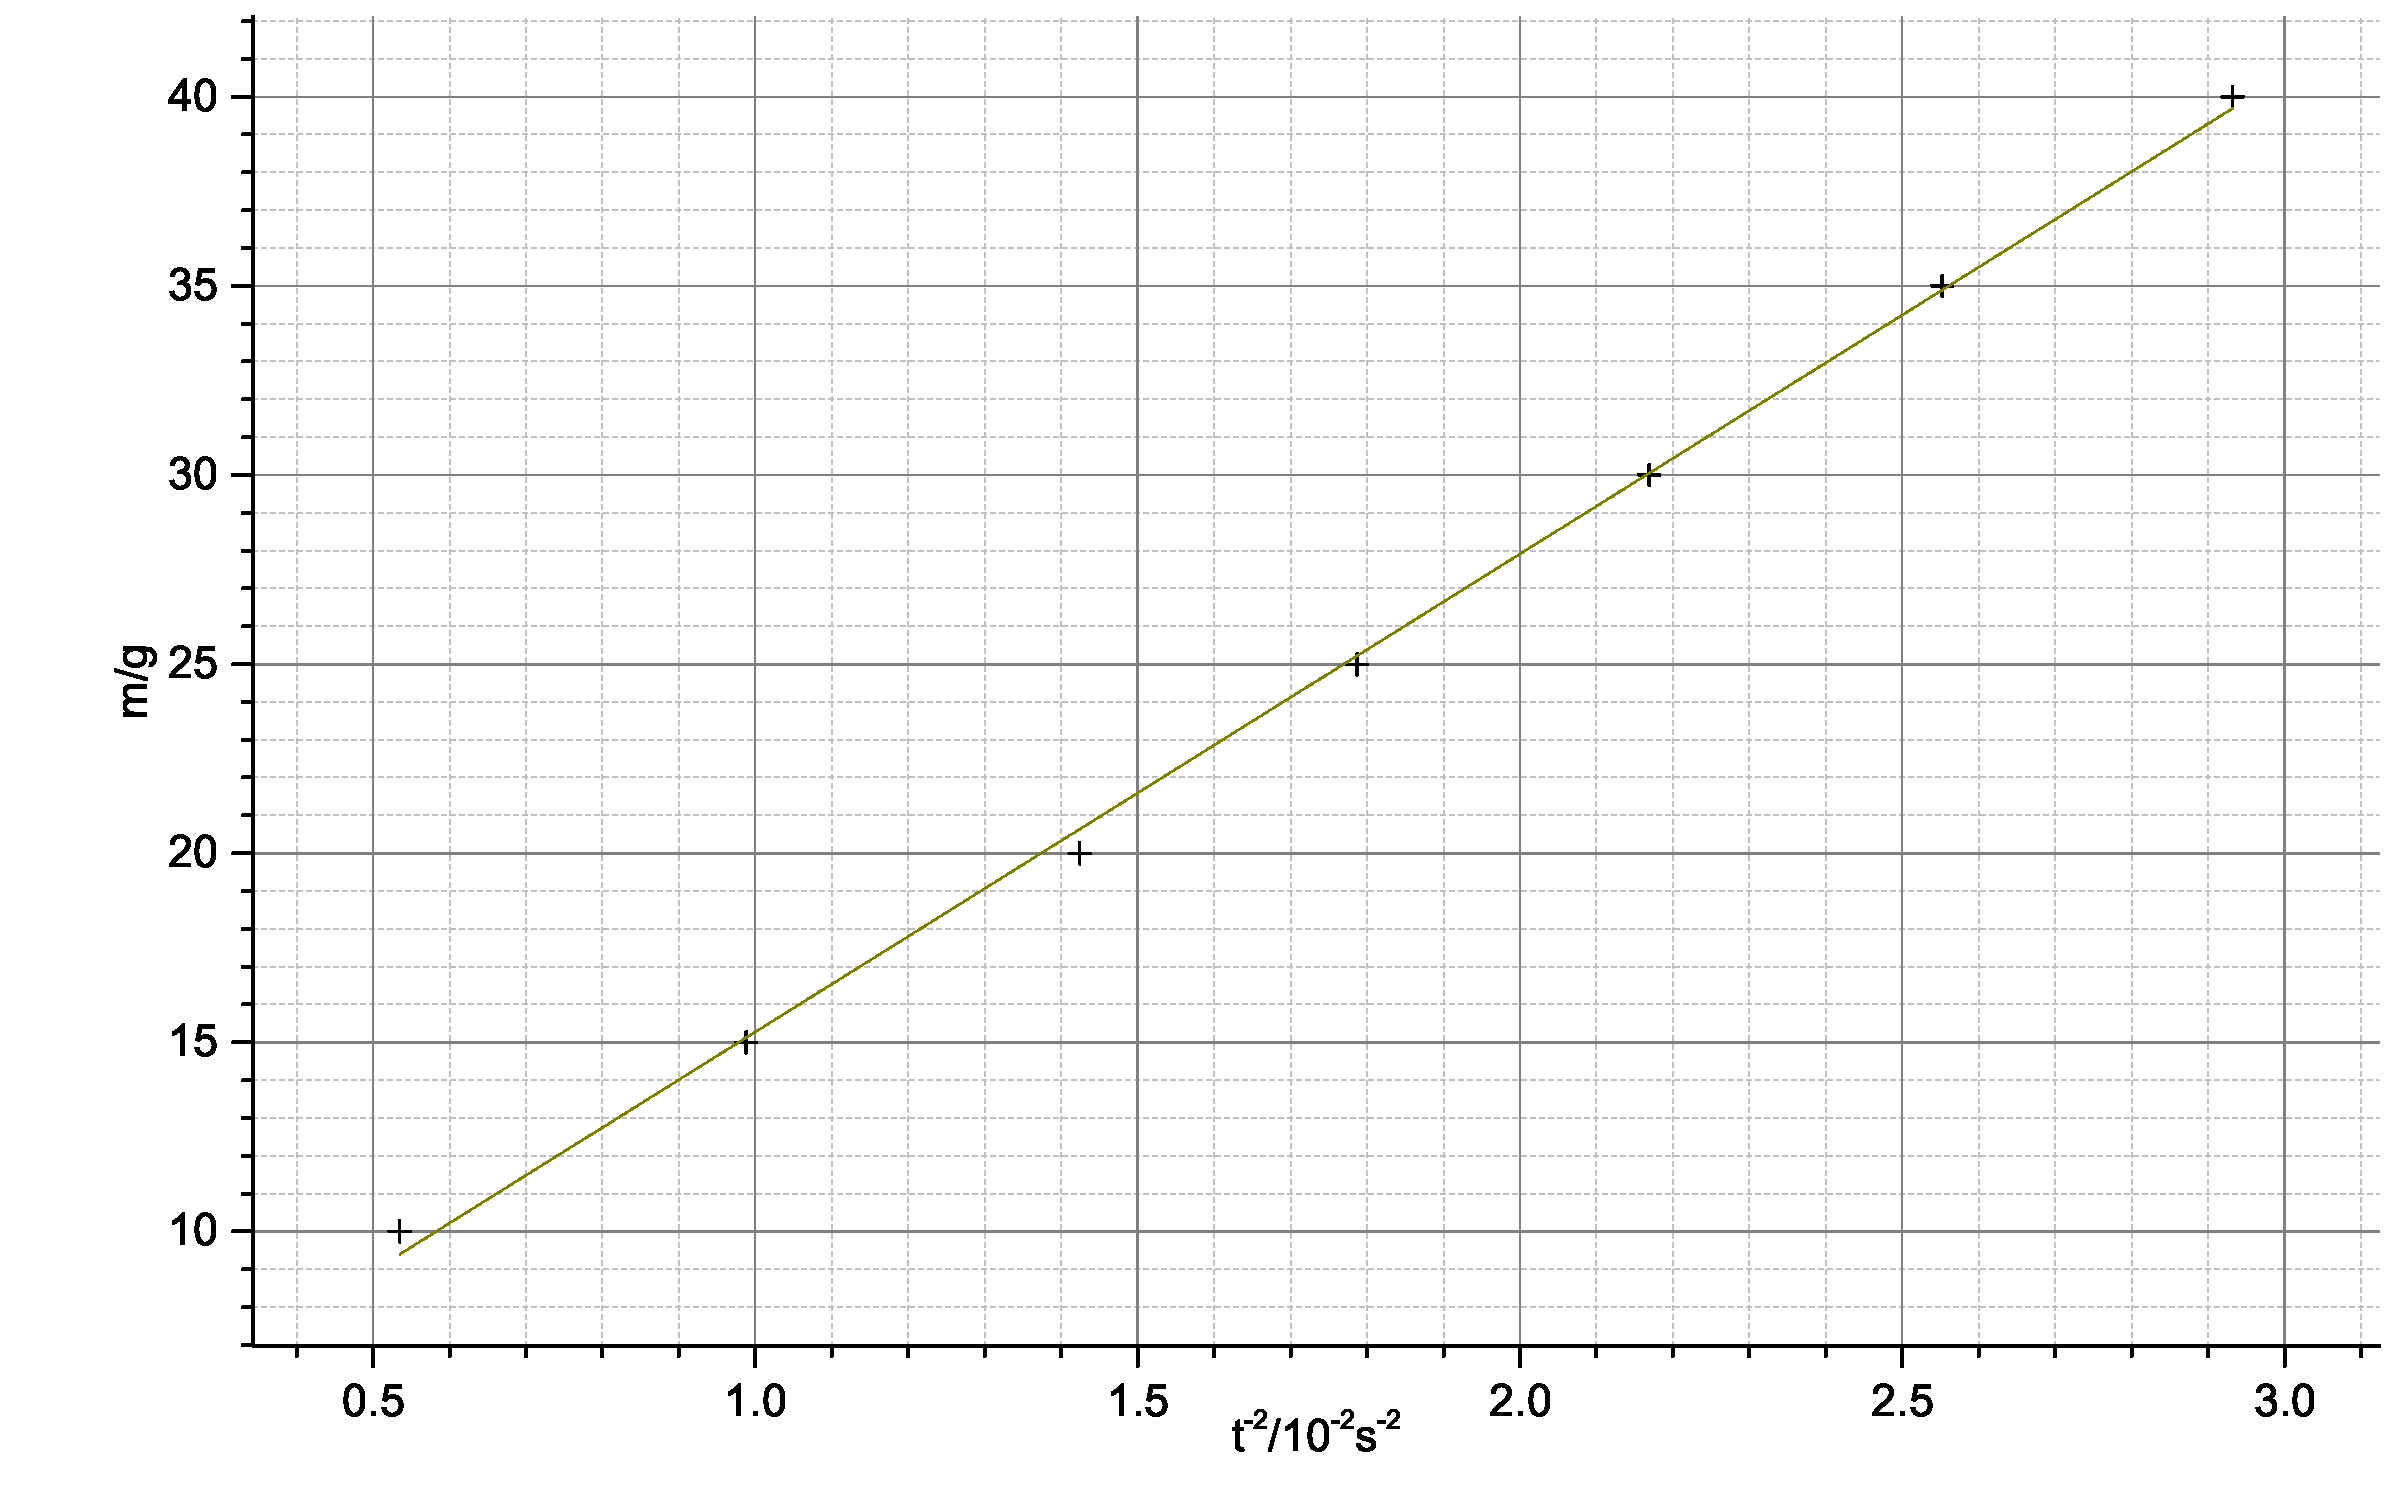
\includegraphics[width=\linewidth,keepaspectratio=true]{m-t.eps}
  \caption{$m-t^{-2}$关系图。从图中可见二者确实成线性关系。}
\end{figure}

对上表中的数据作线性回归分析。以$m$为自变量$x$,$1/t^2$为因变量$y$作最小二乘法,得到

\begin{gather}
  k_2= \frac{\overline{xy}-\bar{x}\bar{y}}{\bar{x^2}-\bar{x}^2}=(52.14214-1.76957\times25)/(725-25^2)=\SI{0.079e-2}{\second^{-2}\gram^{-1}}\\
  b_2= \bar{y}-k_2\bar{x}=1.76957-0.079\times25=\SI{-0.206e-2}{\per\second\squared}\\
  r=\frac{\overline{xy}-\bar{x}\bar{y}}{\sqrt{(\bar{x^2}-\bar{x}^2)(\bar{y^2}-\bar{y}^2)}}=\frac{52.142-1.76957\times25}{\sqrt{3.7568-1.7695^2}\sqrt{725-25^2}}=0.99933
\end{gather}

以$1/t^2$为自变量$y$,$m$为因变量$x$作最小二乘法,得到
\begin{gather}
  k_1= \frac{\overline{xy}-\bar{x}\bar{y}}{\bar{y^2}-\bar{y}^2}=(52.14214-1.76957\times25)/(725-25^2)=\SI{12.6e2}{\gram.\second^2}\\
  b_1= \bar{x}-k_1\bar{y}=25-12.62669\times1.76957=\SI{2.64}{\gram}\\
  r=\frac{\overline{xy}-\bar{x}\bar{y}}{\sqrt{(\bar{x^2}-\bar{x}^2)(\bar{y^2}-\bar{y}^2)}}=0.99933
\end{gather}

显然两种算法得到的相关系数$r$是一样的,因为$r$的表达式中自变量与因变量的地位完全对等。而从$k_1$与$k_2$的定义式中容易得出它们满足关系
\begin{equation}
k_1k_2=\frac{(\overline{xy}-\bar{x}\bar{y})^2} {(\bar{x^2}-\bar{x}^2)(\bar{y^2}-\bar{y}^2)}=r^2
\end{equation}
\end{document} 